\documentclass[addpoints,12pt]{exam}
%\documentclass[12pt]{article}
\usepackage[letterpaper, margin=0.75in]{geometry}
\usepackage{graphicx}
\usepackage{enumitem}
\usepackage{booktabs}
\usepackage{tabularx}

\begin{document}
\footer{}{Page \thepage\ of \numpages}{}

\begin{flushright}
\makebox[0.5\textwidth]{\large Name:\enspace\hrulefill}
\vspace{0.2in}

\makebox[0.5\textwidth]{\large Date:\enspace\hrulefill}
\end{flushright}

\begin{center}

\includegraphics[width=10cm]{../images/logo.png}
\end{center}

\begin{center}
\noindent{\LARGE Conceptual Physics \\ Homework Packet 6 \\}
\end{center}

\noindent\begin{large}\textbf{Due: May 11, 2018}\end{large}
\vspace{0.2in}

Answer the questions in the spaces provided on the question sheets. If you run out of room for an answer, continue on the back of the page. If questions are taken from one of the textbooks, it will be indicated. A large portion of your grade will be calculated based on \textit{how} you obtained an answer, so please \textbf{show your work} (including all diagrams and drawings if relevant).

If you prefer working on loseleaf paper, or have a large portion of your work on loseleaf, please be sure to hand that in along with this homework packet.

The content in this homework relates to quantum mechanics and probability. The related readings are:
\begin{enumerate}
	\item Chapter 33 (Sections 1, 2, 4) of \textit{Light and Matter}
	\item Chapter 34 (Section 1 to 3) of \textit{Light and Matter}
	\item Chapter 35 (Section 1) of \textit{Light and Matter}
\end{enumerate}
 
\clearpage

\begin{flushright}
Score: \hspace{0.2in} / \numpoints ~ points
\end{flushright}

\begin{questions}
\question[6] Suppose you have a fair coin (\textit{i.e.} $P(\textrm{heads}) = 0.5$, $P(\textrm{tails}) = 0.5$).
\begin{parts}
\part What are the sixteen possible outcomes to tossing the coin four times? You can abbreviate, \textit{e.g.} HHTH as opposed to ``two heads followed by one tails followed by one heads.''
\vspace{2in}
\part What is the probability of getting all tails?
\vspace{1in}
\part What is the probability of getting two heads and two tails in no particular order?
\vspace{1in}
\end{parts}

\question[2] If a radioactive substance has a half-life of one year, does this mean that it will be completely decayed after two years? Explain.

From \textit{Light and Matter,} Chapter 33 Question 1.

\fillwithlines{2in}

\clearpage

\question[6] Suppose you have a sample of a radioactive substance that has a half-life of one year.
\begin{parts}
\part What fraction of the sample will have decayed after one year?
\vspace{1in}
\part What fraction of the sample will have decayed after two years?
\vspace{1in}
\part What fraction of the sample will have decayed after five years?
\vspace{1in}
\end{parts}

\question[2] Three particles are traveling at the \textbf{same speed}. The waves of the three particles are as shown.
	\begin{center}
		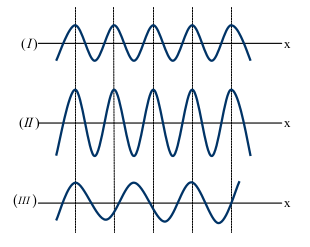
\includegraphics[width=3in]{../images/deBroglie.png}
	\end{center}
	Rank the \textbf{masses} of the particles ( I ), ( II ) and ( III ) by circling one of these six possibilities.
\begin{parts}
	\part $m_{II} > m_I > m_{III}$
	\part $m_{II} > m_{III} > m_I$
	\part $m_{I} = m_{II} > m_{III}$
	\part $m_{I} = m_{II} < m_{III}$
	\part $m_{II} > m_I = m_{III}$
	\part $m_{II} < m_I = m_{III}$
\end{parts}

\clearpage

\question[4] A nuclear physicist is studying a nuclear reaction caused in
an accelerator experiment, with a beam of ions from the accelerator
striking a thin metal foil and causing nuclear reactions when a nucleus from one of the beam ions happens to hit one of the nuclei in
the target. After the experiment has been running for a few hours,
a few billion radioactive atoms have been produced, embedded in
the target. She does not know what nuclei are being produced, but
she suspects they are an isotope of some heavy element such as Pb,
Bi, Fr or U. Following one such experiment, she takes the target foil
out of the accelerator, sticks it in front of a detector, measures the
activity every 5 min, and makes a graph (bottom figure). Which element is it, given the following options? \textbf{Please explain your reasoning.}

From \textit{Light and Matter}, Chapter 33 Question 8


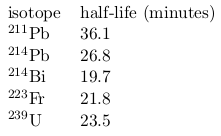
\includegraphics[height=1in]{../images/Isotopes.png}

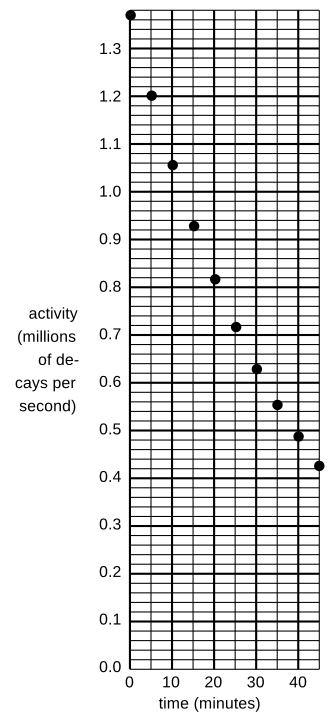
\includegraphics[height=6in]{../images/decay.png}

\clearpage

%\question[4] When light is reflected from a mirror, perhaps only 80\% of the energy comes back. The rest is converted to heat. One could try to explain this in two different ways: (1) 80\% of the photons are reflected, or (2) all the photons are reflected, but each loses 20\% of its energy. Based on your everyday knowledge about mirrors, how can you tell which interpretation is correct?

%From \textit{Light and Matter}, Chapter 34 Question 3
\end{questions}



\end{document}